% !BIB program = bibtex
%%%%%%%%%%%%%%%%%%%%%%%%%%%%%%%%%%%%%%%%%%%%%%%%%%%%%%%
%%% LATEX FORMATTING - LEAVE AS IS %%%%%%%%%%%%%%%%%%%%
\documentclass[11pt]{article} % documenttype: article
\usepackage[top=20mm,left=20mm,right=20mm,bottom=15mm,headsep=15pt,footskip=15pt,a4paper]{geometry} % customize margins
\usepackage{times} % fonttype
\usepackage{listings}
\usepackage{csquotes}
\usepackage{graphicx}
\usepackage{subcaption}
\usepackage[backend=bibtex, sorting=none]{biblatex}

\addbibresource{shifei_chen_assignment_3.bib}
\graphicspath{ {./images/} }

\makeatletter         
\def\@maketitle{   % custom maketitle 
\begin{center}
{\bfseries \@title}
{\bfseries \@author}
\end{center}
\smallskip \hrule \bigskip }

%%%%%%%%%%%%%%%%%%%%%%%%%%%%%%%%%%%%%%%%%%%%%%%%%%%%%%%%%%%%%%%%%%%%
%%% MAKE CHANGES HERE %%%%%%%%%%%%%%%%%%%%%%%%%%%%%%%%%%%%%%%%%%%%%%
\title{{\LARGE Natural Language Processing: Assignment 3}\\[1.5mm]} % Replace 'X' by number of Assignment
\author{Shifei Chen} % Replace 'Firstname Lastname' by your name.

%%%%%%%%%%%%%%%%%%%%%%%%%%%%%%%%%%%%%%%%%%%%%%%%%%%%%%%%%%%%%%%%%%%%
%%% BEGIN DOCUMENT %%%%%%%%%%%%%%%%%%%%%%%%%%%%%%%%%%%%%%%%%%%%%%%%%
%%% From here on, edit document. Use sections, subsections, etc.
%%% to structure your answers.
\begin{document}
\maketitle

\section{Dependency Annotation}

Here are three typical errors I have made during my manual annotation.

\subsection{\texttt{nmod} vs \texttt{compound}}

\begin{displayquote}
  "If a Turkish employee quits, then the Turkish work councils come."
\end{displayquote}

The ambiguation between a single \texttt{nmod} and a \texttt{compound} noun is confusing to me. In the phrase "work councils" I have annotated "work" as a nominal modifier to "councils" while the golden standard says they should be compounded. A compound word usually consists of nouns (or verbs, adjectives, etc.) being writted closely to each other. In fact in some Language like Swedish people usually write them together, without whitespaces. Meanwhile a nominal modifier is usually used to describe an attribute or genitive complement\cite{NmodUD}. In this case, "work" can be argued to be the attribute of "councils" but since this is an idiom\cite{WorksCouncilWiki} so I agree with the golden standard.

\subsection{\texttt{mark}}

\begin{displayquote}
  "National reaction to the events in Kansas demonstrated how deeply divided the country had become."
\end{displayquote}

Here I have marked the word "how" as a \texttt{mark} to the head word "become" rather than an \texttt{advmod} to the head word "deeply". In this sentence, "how deeply divided the country had become" is a complement clause, acting as the object to the verb "demonstrated". The word "become" is a \texttt{ccomp} to "demonstrated"\cite{CcompUD}. The clause has indicated that its object is "divided", not "how", hence we should consider "how" as an adverbial modifer to the other adverb "deeply", even though sometimes "how" can be the mark word of a complement clause\cite{MarkUD}.

\subsection{Subjects in Passive Voice}

\begin{displayquote}
  "The RHS collected comments sent in by schoolchildren and teachers involved in the experiment."
\end{displayquote}

I annotated "sent" to be (\texttt{acl}), the clause modifier of a noun, to "collected" and "schoolchildren" to be the nominal subject of "comments". The error in the former situation is obvious since "collected" is a verb\cite{AclUD}. I should have annotated "sent" to be the \texttt{acl} of "comments". The latter is also wrong. By the meaning of the sentence, it might be intriguing to annotate "schoolchildren" as a \texttt{nsubj} because those children are the one who sent comments. But there is an example from Universal Dependency  explicly says "(\texttt{obl} is used) for the agent of a passive verb (with the optional subtype \texttt{obl:agent}):"\cite{OblUD}. We should mark "schoolchildren" as the \texttt{obl} to the verb "sent".

\section{Dependency Parsing}

Below are two examples of errors made by the parser in Lab 9.

\begin{displayquote}
  A witness told police that the victim had attacked the suspect in April.
\end{displayquote}

In this sentence my parser annotated "police" as the \texttt{obj} of the verb "told", which should be an \texttt{iobj}. "Tell" can have a direct object like in the verb phrase "tell a lie" but here "police" is not the subject, the clause beginning with "that" is. This might be caused by our corpus containing too many "tell"s having direct objects. Also as my parser is a transition based parser, it always has a limited scope of words. It couldn't foresee the words behind "police" therefore it prefered "tell" to have a direct object. Nevertheless UD has a specific label \texttt{iobj} for this kind of indirect subject\cite{IobjUD} and we should stick to that.

The problem of limited scope of words can also be demonstrated by another example in Figure \ref{fig1:limitedscope}.

\begin{figure}[ht]
  \centering
  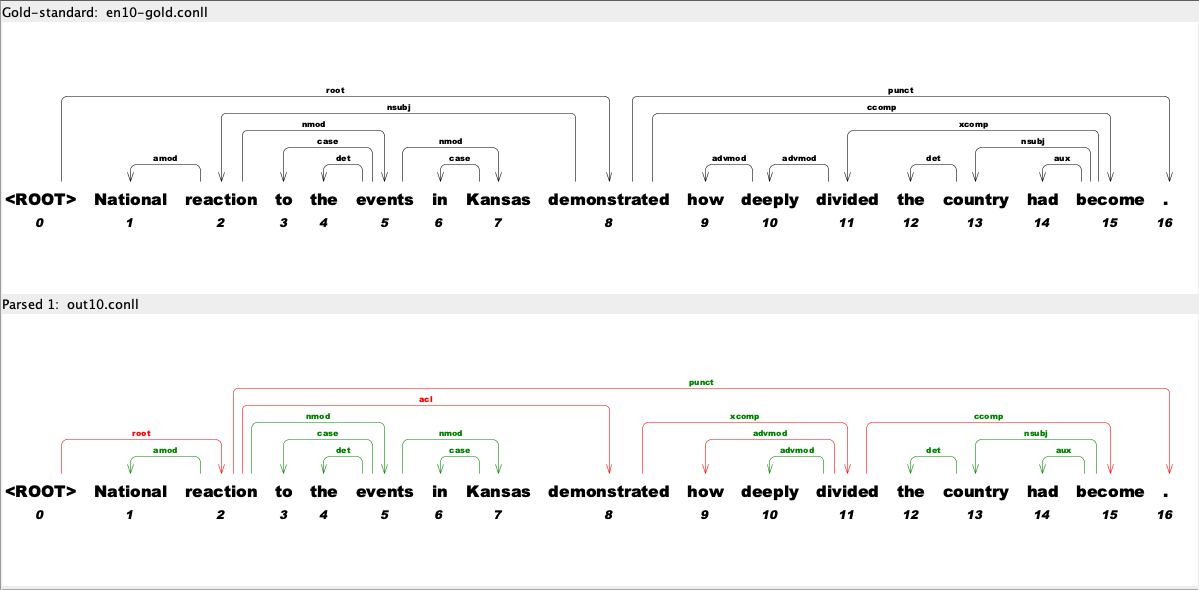
\includegraphics[width=0.9\textwidth]{images/figure_limited_scope.png}
  \caption{The Problem of Limited Scope}
  \label{fig1:limitedscope}
\end{figure}

My parser mistook the main structure of the sentence: it believed "reaction" is the root therefore it continued to make further mistakes. I think this is the case of "error propagation". An arc-eager transition based parser was designed to do some greedy step to build arcs in order to save space in its stack, especially for sentences where the root word is located in the further back.

A transition based depnedency parser has three elements: a stack $S$, a buffer $B$ for unprocessed words and a list $A$ for arcs it has built. Starting with the root word in $S$, it scans the sentence from left to write and makes predictions learned from machine learning about whether to build a left arc or a right arc, to pop a word in the stack (reduce) or to push a word from the buffer to the stack (move). The termination point is when the parser empties its buffer and at that time $A$ is the complete list of parsed arcs.

We shall look at this sentence as an example to show how the parser works.

\begin{equation}
  [\texttt{ROOT}]_s [\texttt{He worked for the BBC for a decade .}]_B
\end{equation}
We start with root being our $W_0$.
\begin{equation}
  [\texttt{ROOT He}]_s [\texttt{worked for the BBC for a decade .}]_B
\end{equation}
Shift "He" into $S$
\begin{equation}
  [\texttt{ROOT}]_s [\texttt{worked for the BBC for a decade .}]_B
\end{equation}
Build a left arc from "worked" to "He", label it \texttt{nsubj}.
\begin{equation}
  [\texttt{ROOT worked}]_s [\texttt{for the BBC for a decade .}]_B
\end{equation}
Build a right arc from root to "worked", label it \texttt{ROOT}.
\begin{equation}
  [\texttt{ROOT worked for the}]_s [\texttt{the BBC for a decade .}]_B
\end{equation}
Shift "for" and the.
\begin{equation}
  [\texttt{ROOT worked for}]_s [\texttt{BBC for a decade .}]_B
\end{equation}
Build a left arc from "BBC" to "the", label it \texttt{det}.
\begin{equation}
  [\texttt{ROOT worked}]_s [\texttt{BBC for a decade .}]_B
\end{equation}
Build a left arc from "BBC" to "for", label it \texttt{case}.
\begin{equation}
  [\texttt{ROOT worked BBC}]_s [\texttt{for a decade .}]_B
\end{equation}
Build a right arc from "worked" to "BBC", label it \texttt{obl}.
\begin{equation}
  [\texttt{ROOT worked BBC for a}]_s [\texttt{decade .}]_B
\end{equation}
Shift "for" and "a".
\begin{equation}
  [\texttt{ROOT worked BBC for}]_s [\texttt{decade .}]_B
\end{equation}
Build a left arc from "decade" to "a", label it \texttt{det}.
\begin{equation}
  [\texttt{ROOT worked BBC}]_s [\texttt{decade .}]_B
\end{equation}
Build a left arc from "decade" to "for", label it \texttt{case}.
\begin{equation}
  [\texttt{ROOT worked}]_s [\texttt{decade .}]_B
\end{equation}
Reduce "BBC".
\begin{equation}
  [\texttt{ROOT worked decade}]_s [\texttt{.}]_B
\end{equation}
Build a right arc from "worked" to "decade", label it \texttt{obl}.
\begin{equation}
  [\texttt{ROOT worked}]_s [\texttt{.}]_B
\end{equation}
Reduce "decade".
\begin{equation}
  [\texttt{ROOT worked .}]_s []_B
\end{equation}
Build a right arc from "worked" to ".", label it \texttt{punc}. The empty buffer $B$ marks our end of parsing.

\section{Context-Free Grammar}

My grammar goes as the following one.

\begin{lstlisting}[language=Python, frame=single, showstringspaces=false]
# Grammar
S -> S Punct
S -> NP VP
NP -> NP PP | Det NP | Adj NP
NP -> Pronoun | Pronoun Pronoun | Noun | Noun Cconj Noun
VP -> Aux VP | Adv VP
VP -> Verb NP | Verb SBAR | Verb PP | Verb PP PP
PP -> Prep NP
SBAR -> Sconj S
# Lexicon
Noun -> 'decade' | 'experience' | 'warming' | 'change' | 'pattern' |
  'seasons' | 'part' | 'scheme' | 'money' | 'sponsorship' | 'advertising'
Verb -> 'worked' | 'spoke' | 'caused' | 'wonder' | 'played' | 'makes'
Adj -> 'Global' | 'rainy'
Aux -> 'has'
Adv -> 'also'
Sconj -> 'whether'
Cconj -> 'and'
Pronoun -> 'BBC' | 'He' | 'She' | 'CNN' | 'Style' | 'I' | 'Davis' | 'Cup'
Det -> 'the' | 'a' | 'The'
Prep -> 'for' | 'to' | 'about' | 'in' | 'of' | 'through'
Punct -> '.'
\end{lstlisting}

What I have extended are the rules for noun pharses and verb phrases. A noun phrase can consist of several nouns, pronouns or nouns connected by a coordinating conjunction. In additional it can also consist of a noun followed by one or several prepositional phrases, e.g. "a change in the pattern" and "the fire in December". For verbs they can have nouns, one/several prepositional phrase, or even a subjordinate clause as their object. There are also cases that a verb follows an auxiliary verb like "has caused", or cases that it follows an adverb, like "also wonder", even thought some may argue that the adverb "also" in this case should not be a part of the verb phrase because it modifies the whole sentence, not only the verb.

\begin{figure}[p]
  \centering
  \begin{subfigure}{0.45\textwidth}
    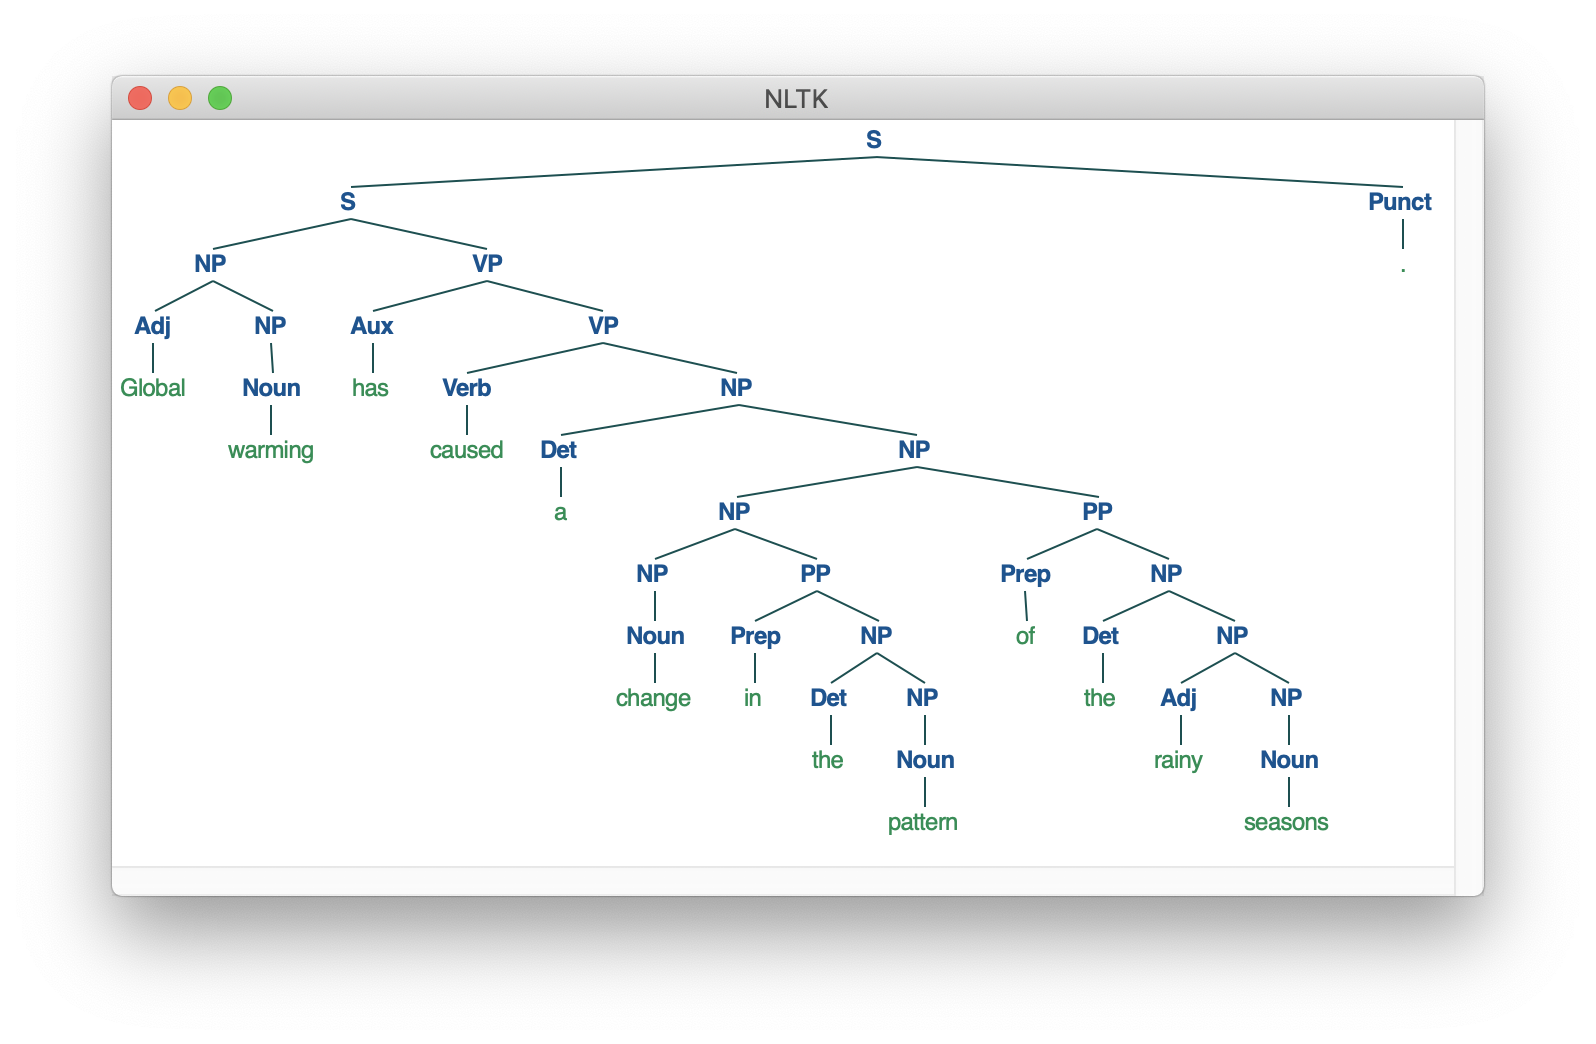
\includegraphics[width=0.9\linewidth]{images/figure_cfg_tree_1.png}
    \caption{}
  \end{subfigure}
  \begin{subfigure}{0.45\textwidth}
    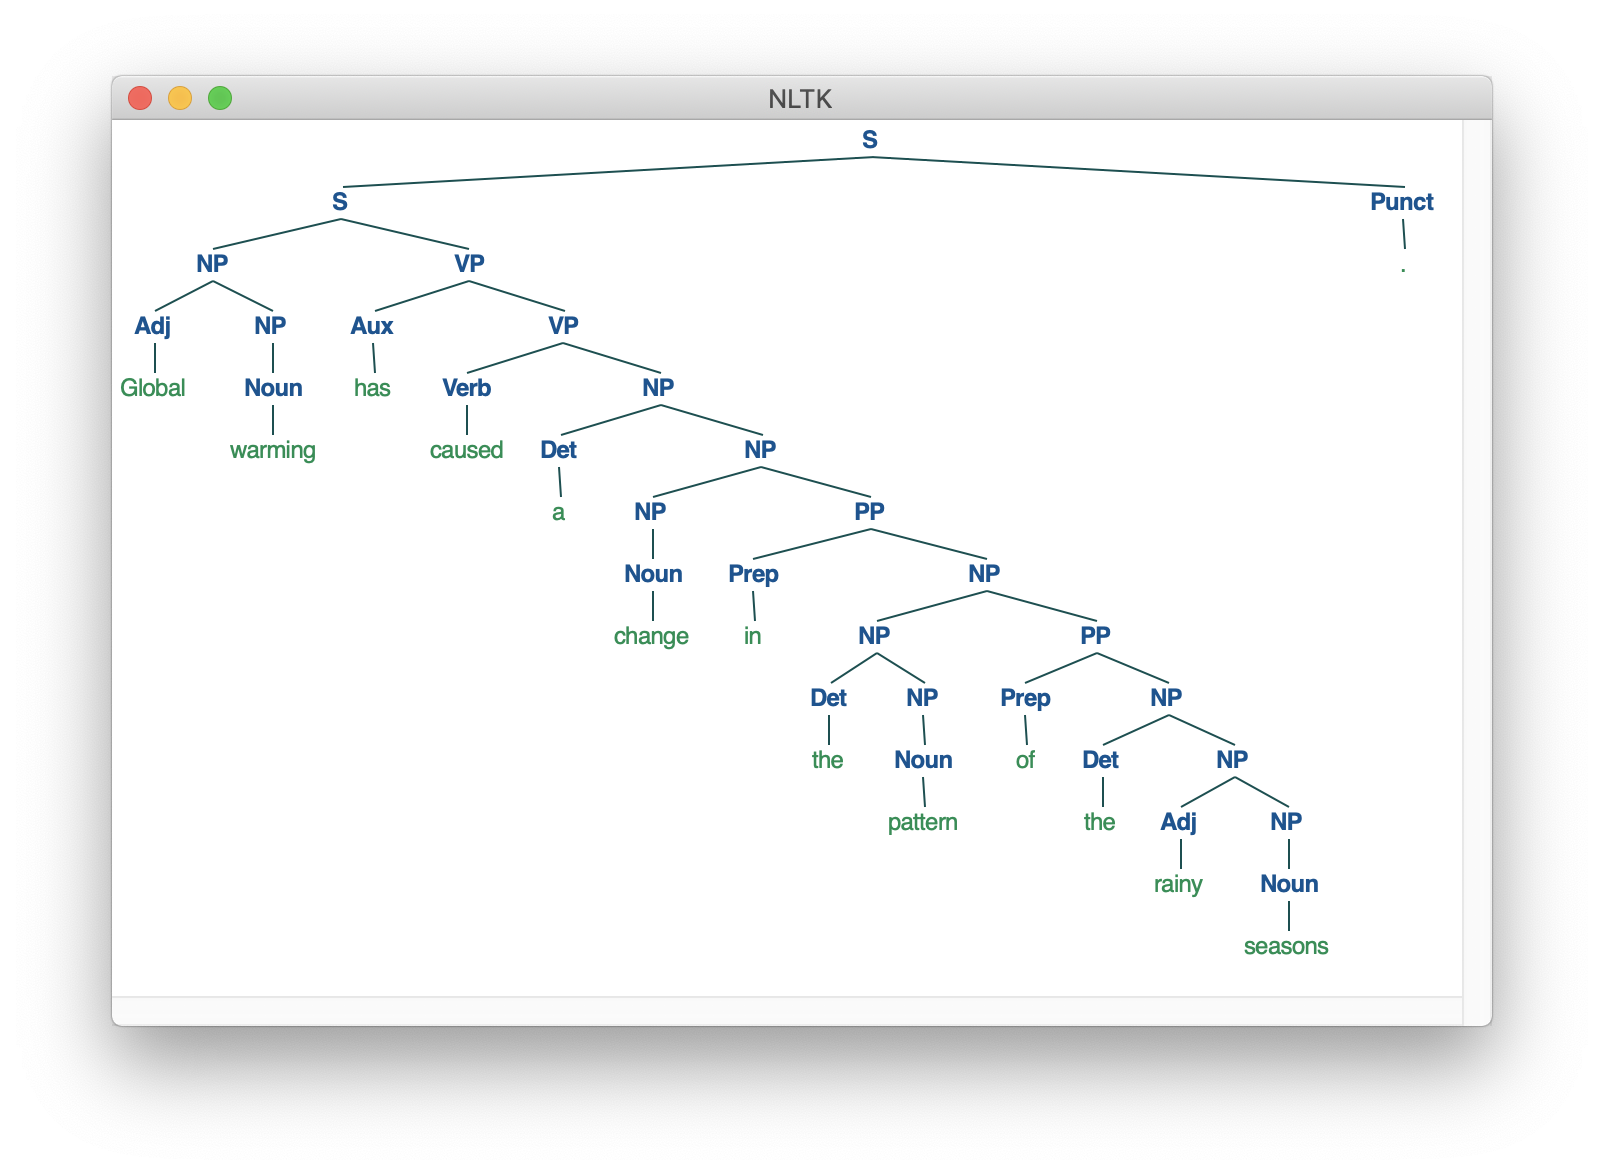
\includegraphics[width=0.9\linewidth]{images/figure_cfg_tree_2.png}
    \caption{}
  \end{subfigure}

  \begin{subfigure}{0.45\textwidth}
    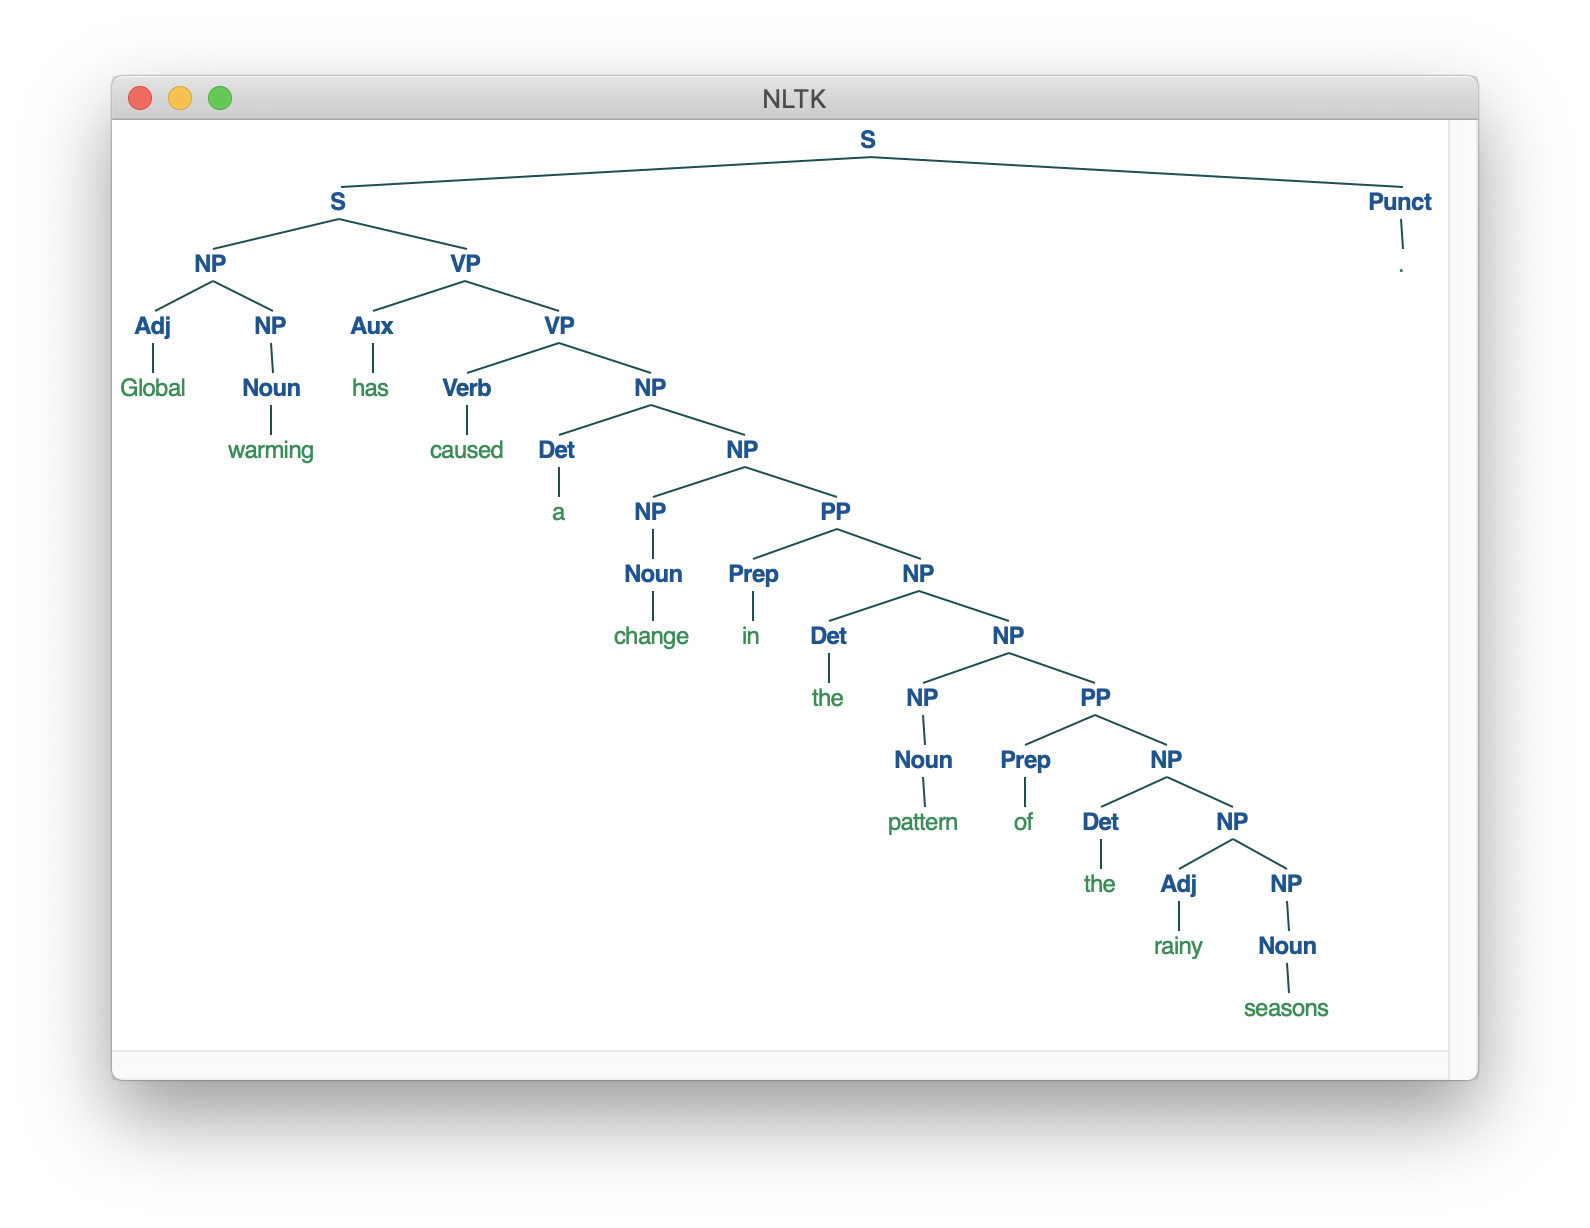
\includegraphics[width=0.9\linewidth]{images/figure_cfg_tree_3.png}
    \caption{}
    \label{fig2:golden}
  \end{subfigure}
  \begin{subfigure}{0.45\textwidth}
    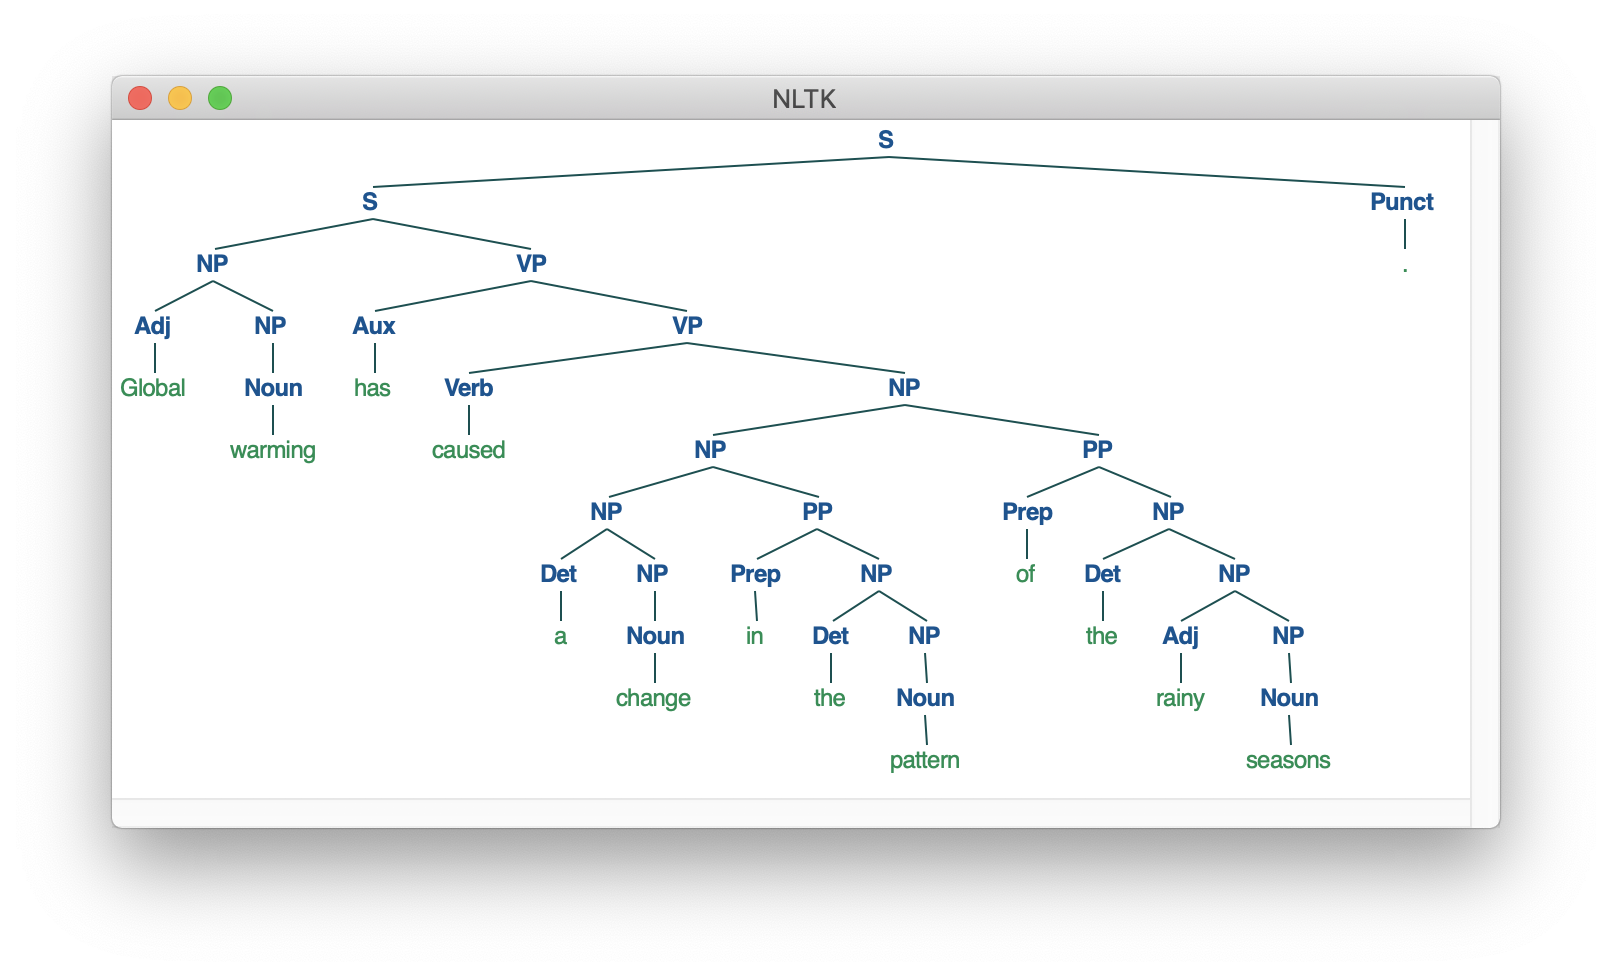
\includegraphics[width=0.9\linewidth]{images/figure_cfg_tree_4.png}
    \caption{}
    \label{fig2:doublepponchange}
  \end{subfigure}
  
  \begin{subfigure}{0.45\textwidth}
    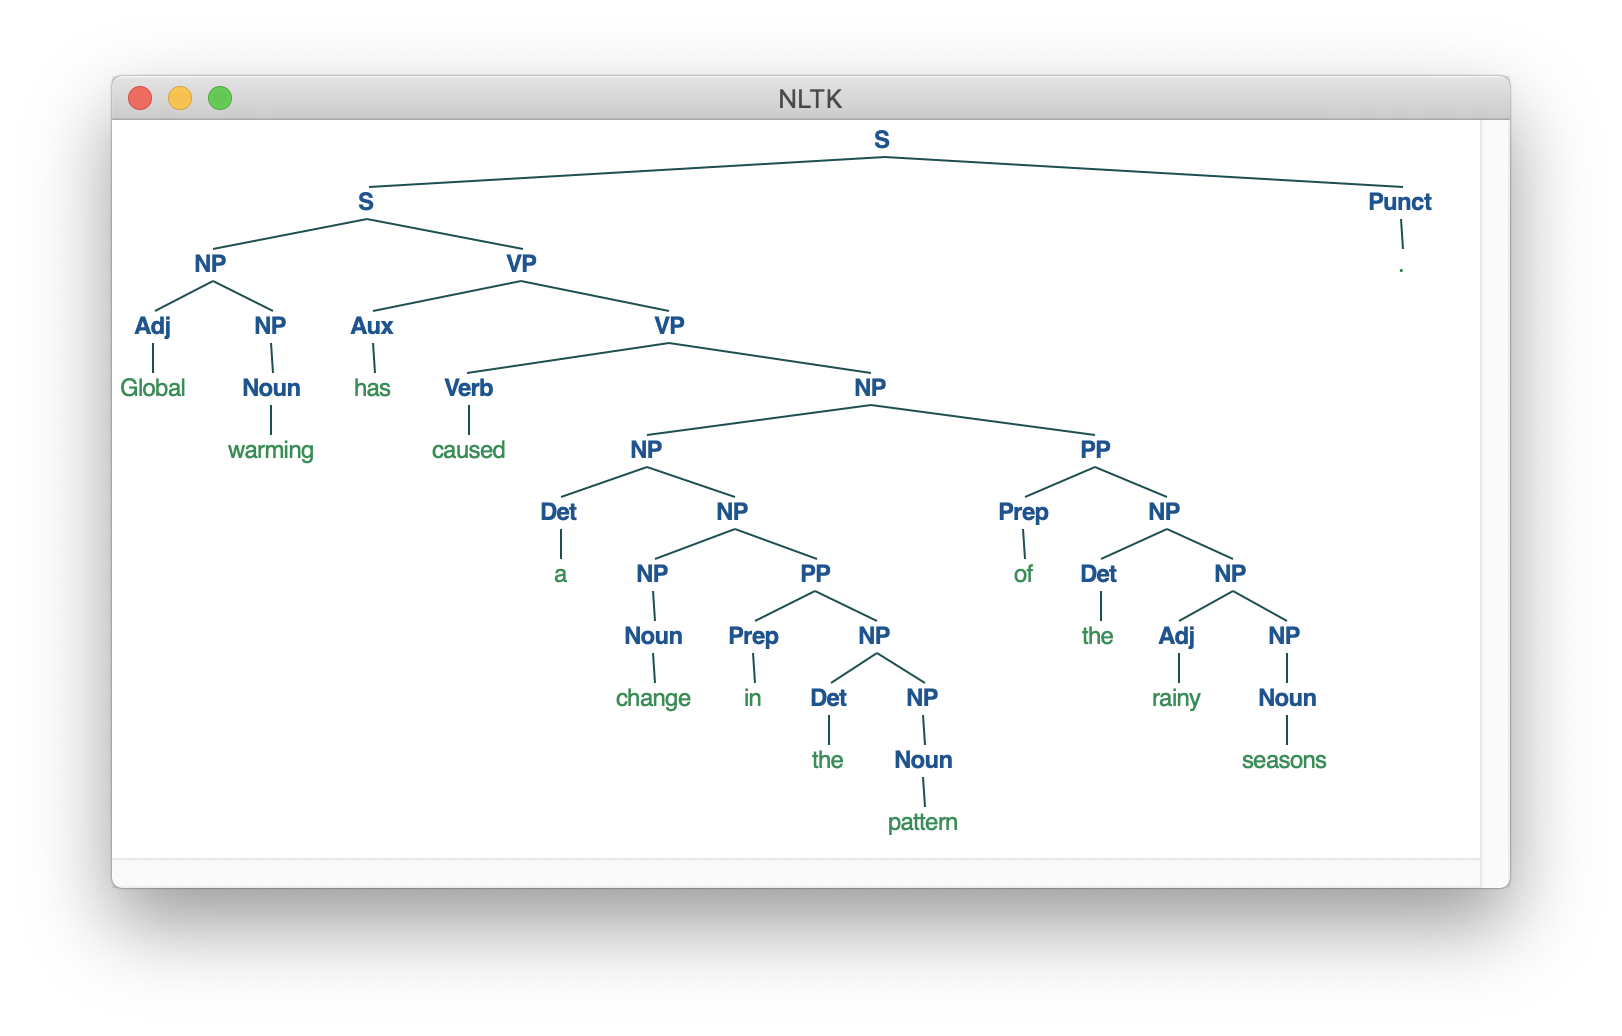
\includegraphics[width=0.9\linewidth]{images/figure_cfg_tree_5.png}
    \caption{}
  \end{subfigure}
  \begin{subfigure}{0.45\textwidth}
    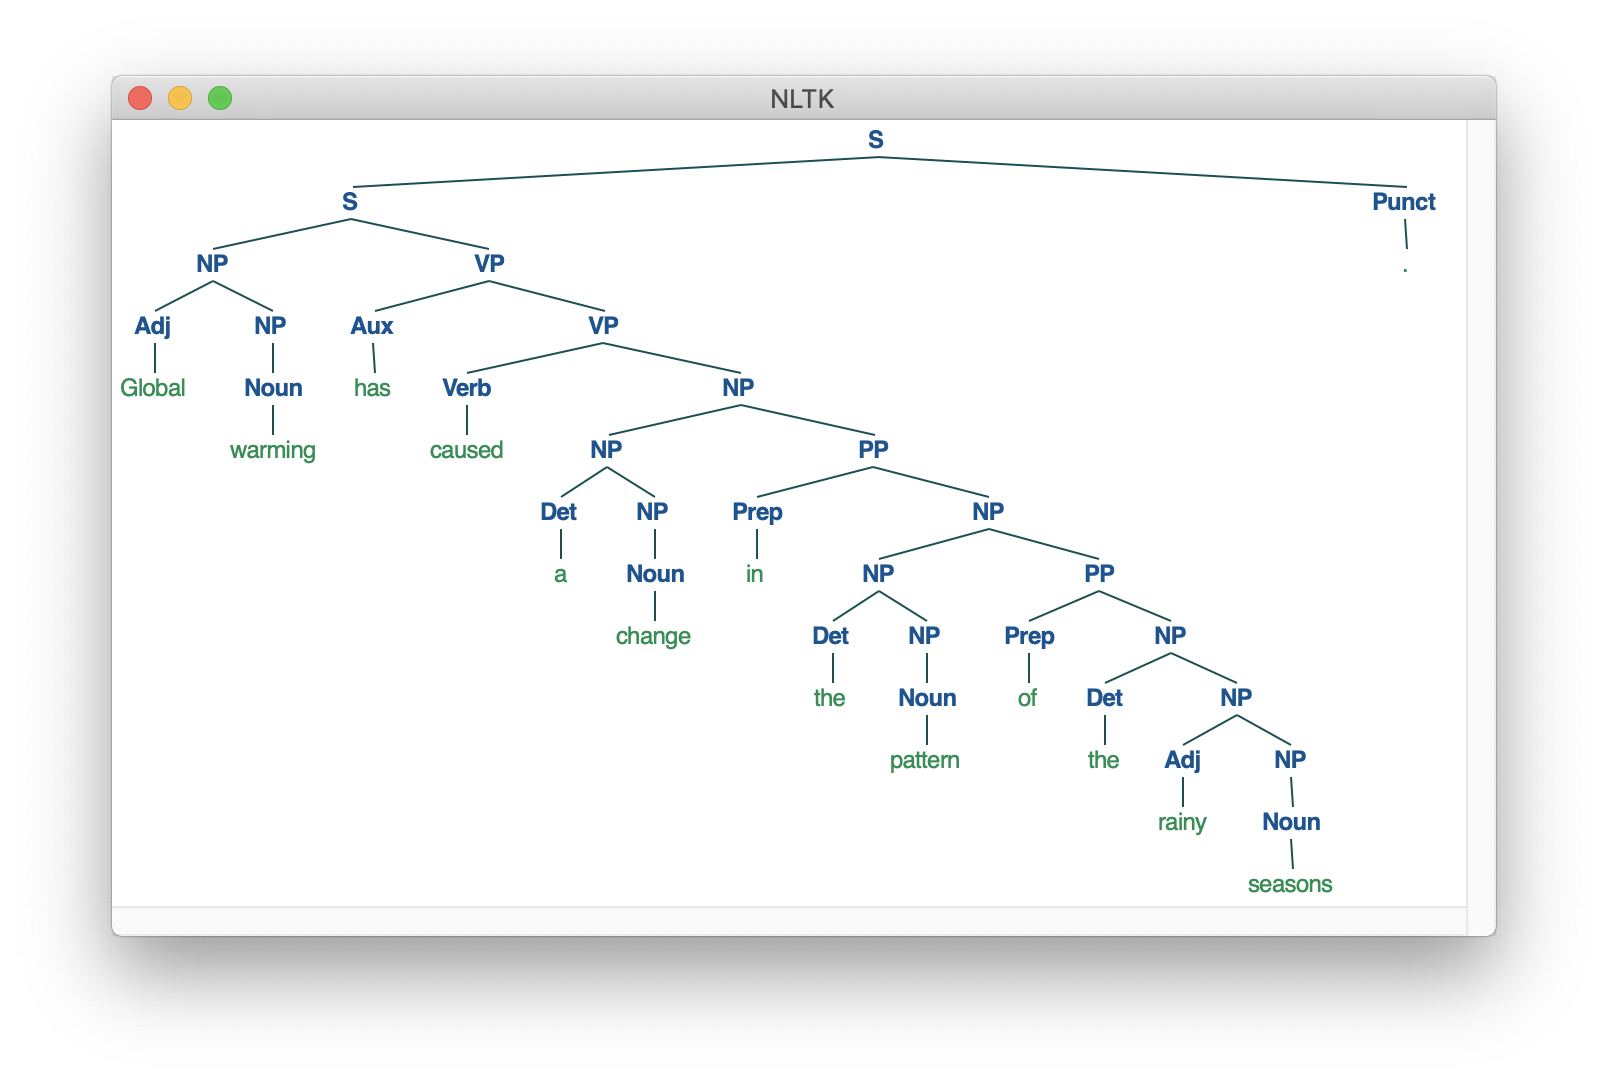
\includegraphics[width=0.9\linewidth]{images/figure_cfg_tree_6.png}
    \caption{}
  \end{subfigure}

  \begin{subfigure}{0.45\textwidth}
    \centering
    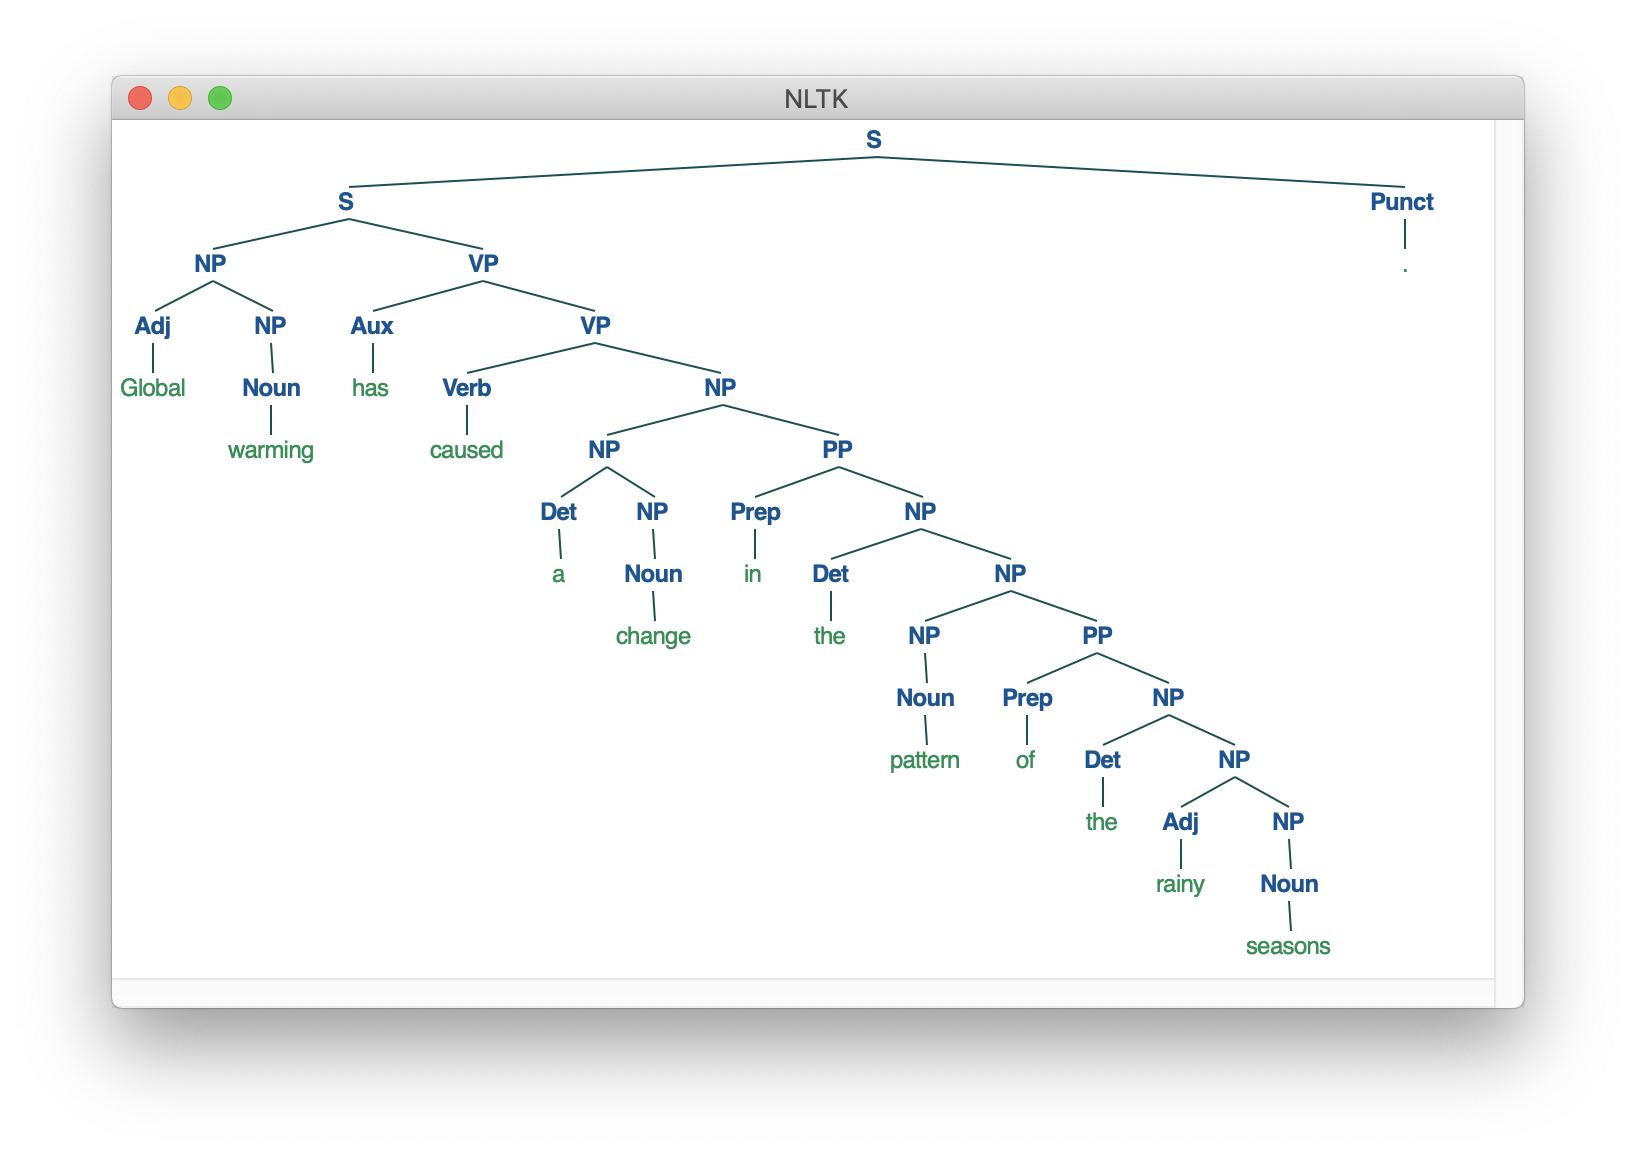
\includegraphics[width=0.9\linewidth]{images/figure_cfg_tree_7.png}
    \caption{}
  \end{subfigure}

  \caption{Different Trees Generated by My Grammar}
  \label{fig2:cfgtrees}
\end{figure}

My grammar has generated 7 different trees for the sentence "Global warming has caused a change in the pattern of the rainy seasons." The left part of the sentence "Global warming has caused" and the punctuation are the same in all trees. They differ in parsing the big \texttt{NP} "a change in the pattern of the rainy seasons". Only one of them(Figure \ref{fig2:golden}) picked "change" to be the head word of "pattern" and "pattern" to be the head word of "seasons", which is what the golden standard did as well. I believe the variety, or ambiguaty is caused by my recursive definition-\texttt{NP} $\rightarrow$ \texttt{NP} \texttt{PP} and \texttt{PP} $\rightarrow$ \texttt{Prep} \texttt{NP}. If we could assign probabilities to each grammar rule then I believe we can disambigute this sentence.

In the lecture we have learned CYK algorithm to parse sentences. In order to apply it, first we need to convert our CFG to the one in Chomsky normal form\cite[436]{JurafskyMartin200805}. After that we draw the upper-right portion of a $(n+1)*(n+1)$ matrix for a $n$ words sentence, each of its cell $[i, j]$ will hold a set of non-terminals representing all of the consitituents spanning from position $i$ through $j$. We first fill out all the cells that are located on the diagonal line by looking for the input in the CNF grammer. The results are usually their corrsponding pos tags. Then we move from left to right in the table and for each column we start at the second but last cell at the bottom all the way to the top. For cell $[i, j]$ we look at cell $[i, x]$ on the left in the same row and the cell $[x, j]$ below in the column to search for the first and the second non-terminals which can be the right-hand part of a rule in our CNF grammar (order matters). We write down the left hand side non-terminal in the cell $[i, j]$. If there are several rules exist, we need to write down all of the possible non-terminals. Then we continue filling up the table until cell $[0, n]$. Figure \ref{fig3:cyk} below is my final table for parsing the sentence "He worked for the BBC for a decade."

\begin{figure}[ht]
  \centering
  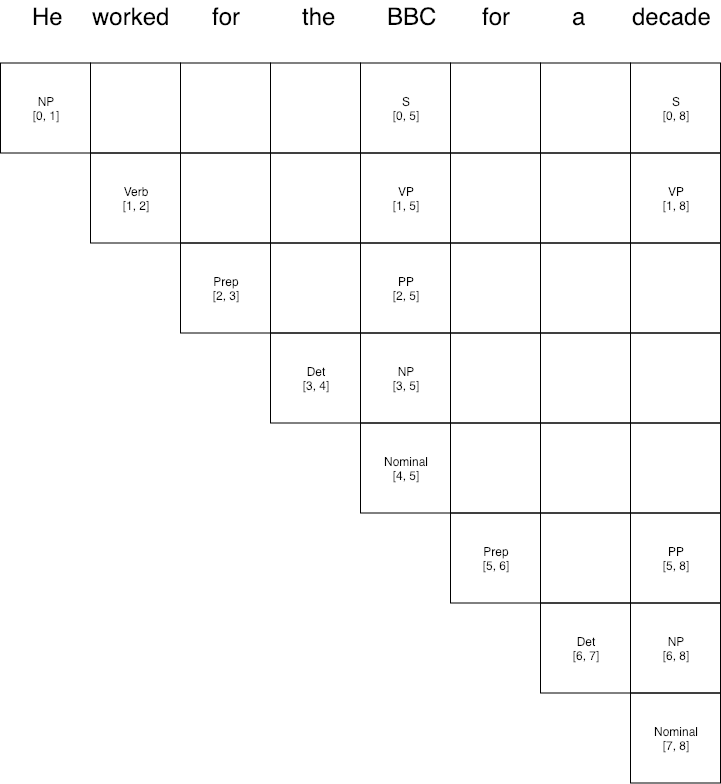
\includegraphics[width=0.9\textwidth]{images/figure_cyk.png}
  \caption{Parsing table by using the CYK algorithm}
  \label{fig3:cyk}
\end{figure}

\printbibliography

\end{document}
